\chapter{XMPP}\label{chap:6}
\section{Servicios de Mensajería}
\subsection{Introducción}

En esta práctica se utilizará el protocolo XMPP{.}
Se utiliza un docker para almacenar el servidor XMPP{.}
Los alumnos crean clientes para interactuar en el servidor mediante mensajes XMPP{.}
Finalmente, se estudia algún aspecto del protocolo y se desarrolla un bot.

\begin{notebox}
Todos los ficheros y configuraciones relacionadas a esta sesión se encuentran en el directorio
\Verb#is-pl3-g1/6_xmpp#.
\end{notebox}

\subsection{Servidores XMPP}
La primera tarea a realizar es instalar el servidor XMPP es un contenedor Docker.
Posteriormente, hemos configurado el fichero \Verb#prosody.cfg.lua#
(localizado en \\ \Verb#{/etc/prosody/prosody.cfg.lua}#).
Escribimos el fichero \lstinline{Dockerfile} que lanza el contenedor de Prosody,
pasándole las carpetas de configuración \Verb#data# y \Verb#/etc/prosody#.
A continuación, hemos creado los certificados necesarios para el servidor, y los extraemos
del contenedor Docker a nuestra carpeta de configuración \Verb#data# (\Verb#{ingserv01.*}#).

Finalmente, hemos dado de alta a dos cuentas de usuario en el servidor Prosody
para que puedan acceder a la aplicación XMPP{.}

Los dos usuarios son:
\begin{itemize}[itemsep=0.10px]
    \item manolo@ingserv01 (conManolo)
    \item ramon@ingserv01 (conRamon)
\end{itemize}

\subsection{Clientes XMPP}
En la distribución de Linux utilizada para instalar el cliente, Debian 12 Bookworm,
se han instalado los paquetes del repositorio oficial \italic{stable}
\Verb#pidgin 2.14.12-1# y \\ \Verb#pidgin-data 2.14.12-1#.

\begin{minipage}{\linewidth}
	\centering
	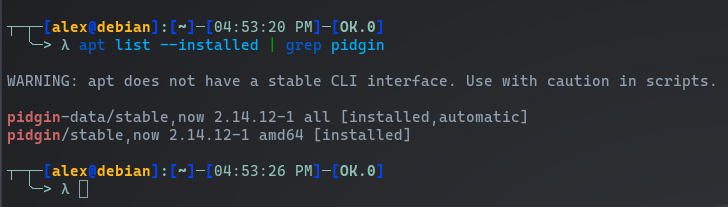
\includegraphics[width=\textwidth]{6/Imagen610.png}
	\captionof{figure}{Paquetes a instalar en Debian 12 Bookworm}\label{fig:6/1}
\end{minipage}

Mediante las herramientas de desarrollador, se aprecia que se descargan fragmentos del vídeo

Hacemos login como ambos usuarios y los añadimos como amigos.
De ahora en adelante, será posible que estos dos usuarios chateen entre ellos.

\begin{minipage}{\linewidth}
	\centering
	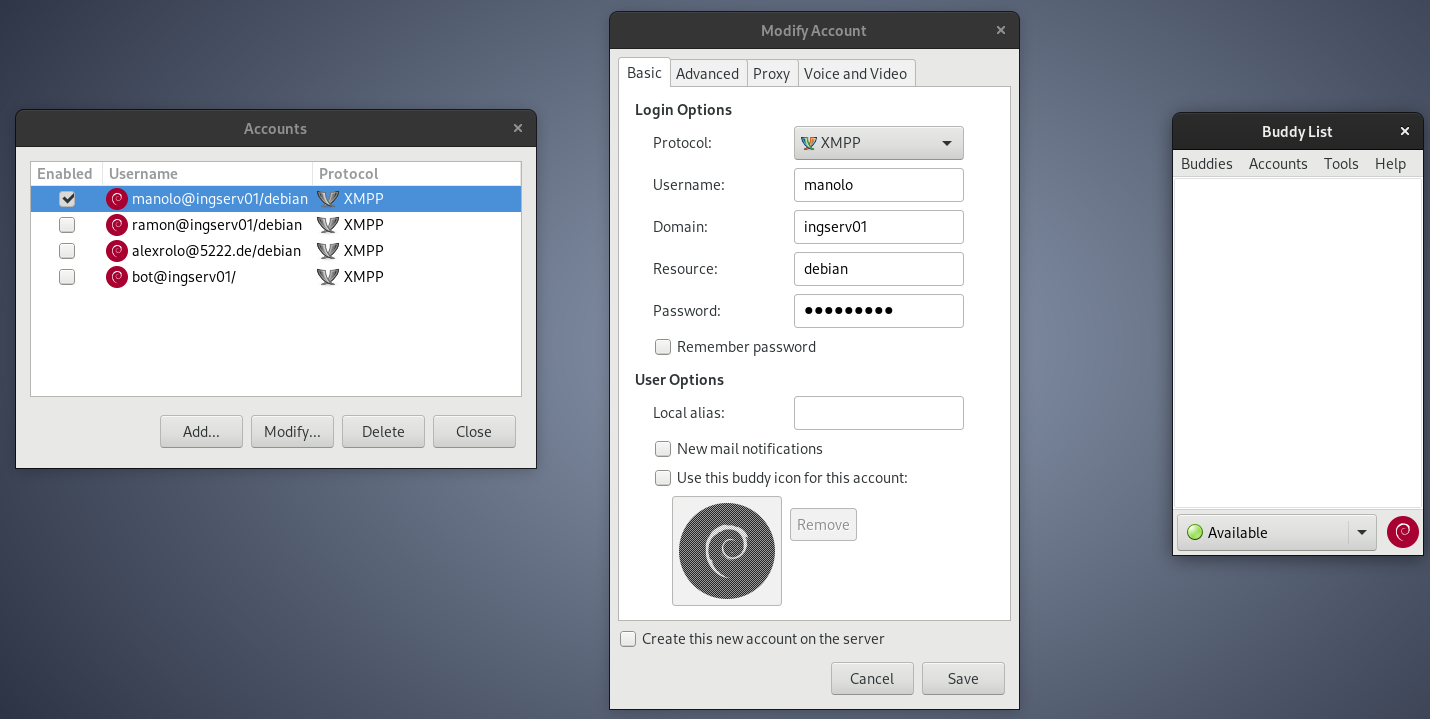
\includegraphics[width=\textwidth]{6/Imagen611.png}
	\captionof{figure}{Login con uno de los usuarios}\label{fig:6/2}
\end{minipage}

Estos dos usuarios se comunican utilizando el programa.

\begin{minipage}{\linewidth}
	\centering
	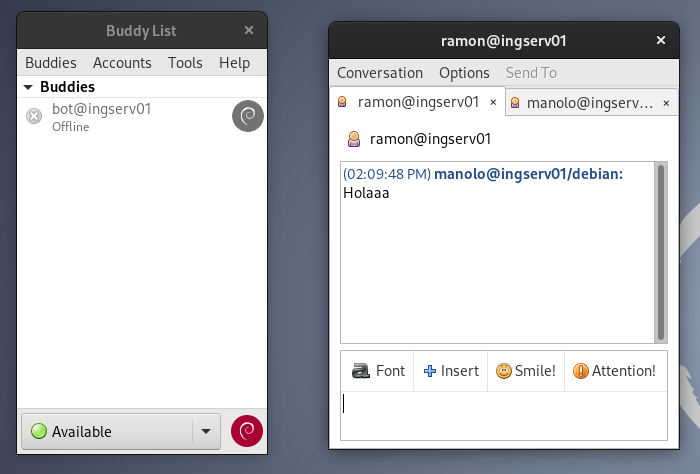
\includegraphics[width=\textwidth]{6/Imagen613.png}
	\captionof{figure}{Chat entre dos usuarios}\label{fig:6/3}
\end{minipage}

\subsection{Protocolo XMPP}
Procedemos a analizar las \italic{stanzas} que recibe la app Pidgin.
Podemos ver las estrofas del \lstinline{ping} que envía Pidgin periódicamente.
También se ven los cambios de estado con la \italic{stanza} presence.
Finalmente, observamos \italic{stanzas} recibidas al enviar un mensaje.

\begin{minipage}{\linewidth}
	\centering
	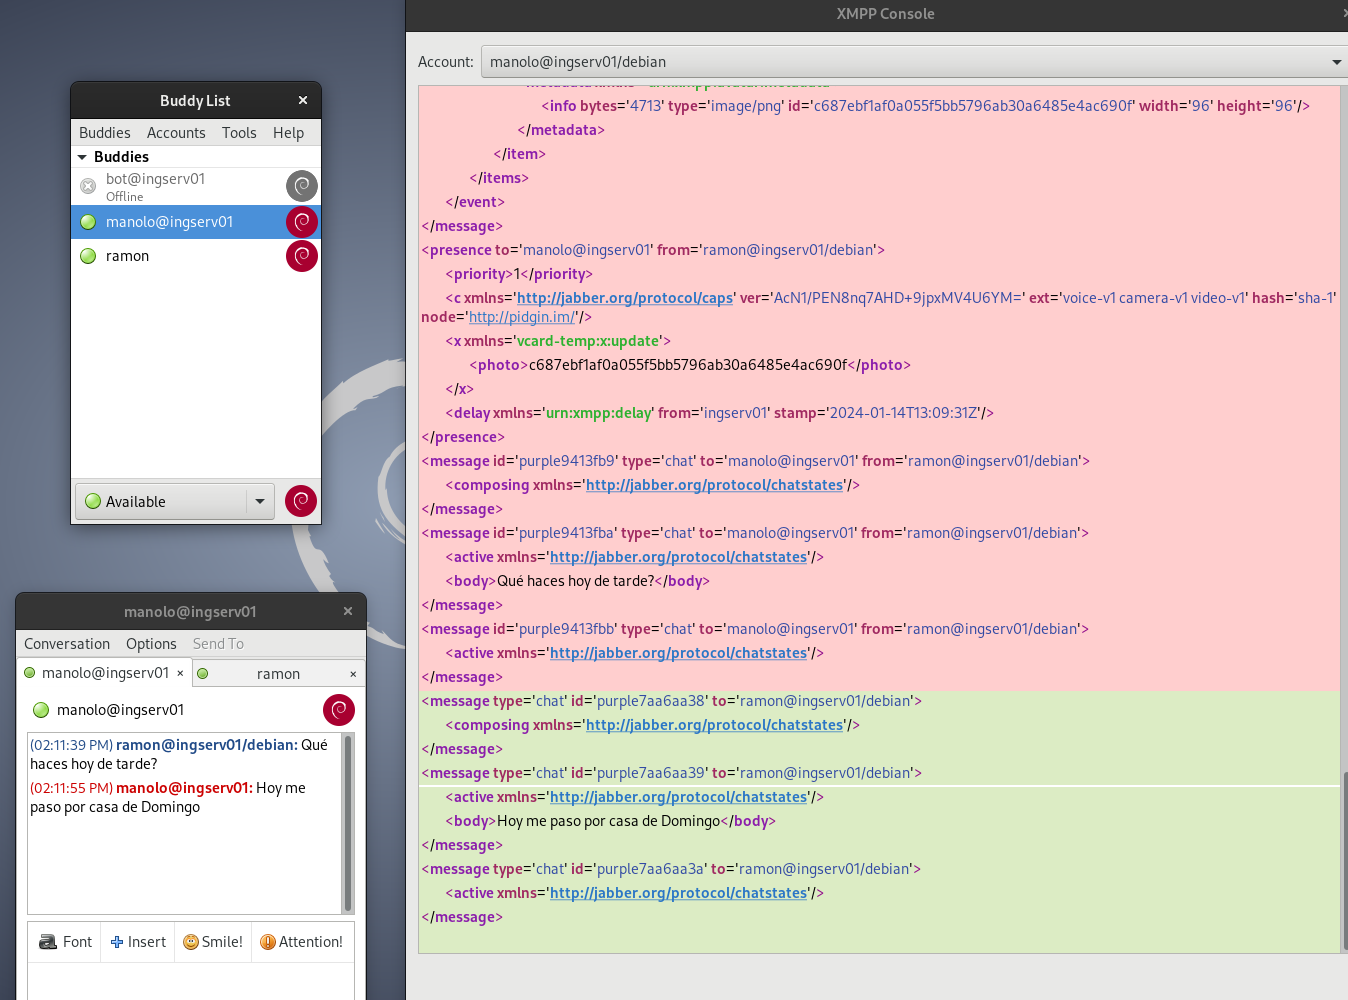
\includegraphics[width=\textwidth]{6/Imagen612.png}
	\captionof{figure}{Mensajes entre dos usuarios}\label{fig:6/4}
\end{minipage}

Igual sucede cuando dos usuarios se subscriben a las notificaciones.

\begin{minipage}{\linewidth}
	\centering
	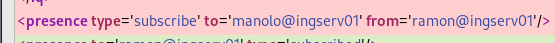
\includegraphics[width=\textwidth]{6/Imagen614.png}
	\captionof{figure}{Subscripción de un usuario a otro}\label{fig:6/5}
\end{minipage}

\subsection{Bot XMPP}
En esta ultima sección desarrollamos un bot XMPP{.}
El bot funcionará como un usuario más en el roster.
Usuarios podrán añadir al bot a su lista de amigos y le podrán enviar mensajes.
Si al bot se le presenta una operación matemática, responderá con el resultado,
mientras que si no es una operación matemática, el bot responderá con el mismo mensaje.

A la hora de desarrollar el bot, nos encontramos con varios problemas.
La libería a utilizar, \Verb#sleekxmpp# no estaba disponible en el repositorio
oficial de Debian y el script de instalación del paquete de \Verb#pip# no funciona correctamente.

Como solución a este problema, decidimos omitir la tarea de desarrollar el bot en local
y proceder directamente a desarrollar el bot en un contenedor Docker.

Al utilizar un contenedor Docker, podemos bajarnos una imagen de una versión de Python que sí soporte
el paquete de \Verb#pip sleekxmpp#.

El \Verb#Dockerfile# utiliza una imagen de Python 3.8
y los paquetes \Verb#wheel# y \Verb#sleekxmpp#.

Una vez hecho esto, hemos comenzado el desarrollo del bot.
Definimos la clase \Verb#Bot# y sus métodos de \Verb#callback#.
Añadimos un método \Verb#main# que crea una nueva instancia del bot
y solicita los parámetros necesarios si no se han pasado previamente
por línea de comandos.

Hemos tenido que añadir dos líneas de código específicas sobre \Verb#SSL#
para que el bot ignore el certificado del servidor.
Si no se añaden estas líneas, nos es imposible ejecutar el bot con exito.

Finalmente, escribimos un fichero \Verb#lanza-bot.sh# con el código necesario
para lanzar el contenedor del bot e iniciar el programa con los parámetros adecuados.

Aquí se muestra un ejemplo de interacción con el bot: \\
\begin{minipage}{\linewidth}
	\centering
	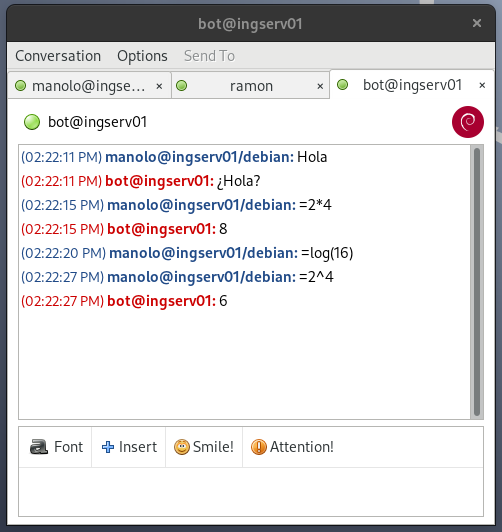
\includegraphics[width=\textwidth]{6/Imagen615.png}
	\captionof{figure}{Comunicación con el bot}\label{fig:6/6}
\end{minipage}

No obstante, al enviar el mensaje \verb#=log(16)#
el bot no sabe qué hacer, por lo que la función \verb#eval#
que utilizamos para resolver las operaciones no tiene todas
las funciones matemáticas definidas.

\begin{minipage}{\linewidth}
	\centering
	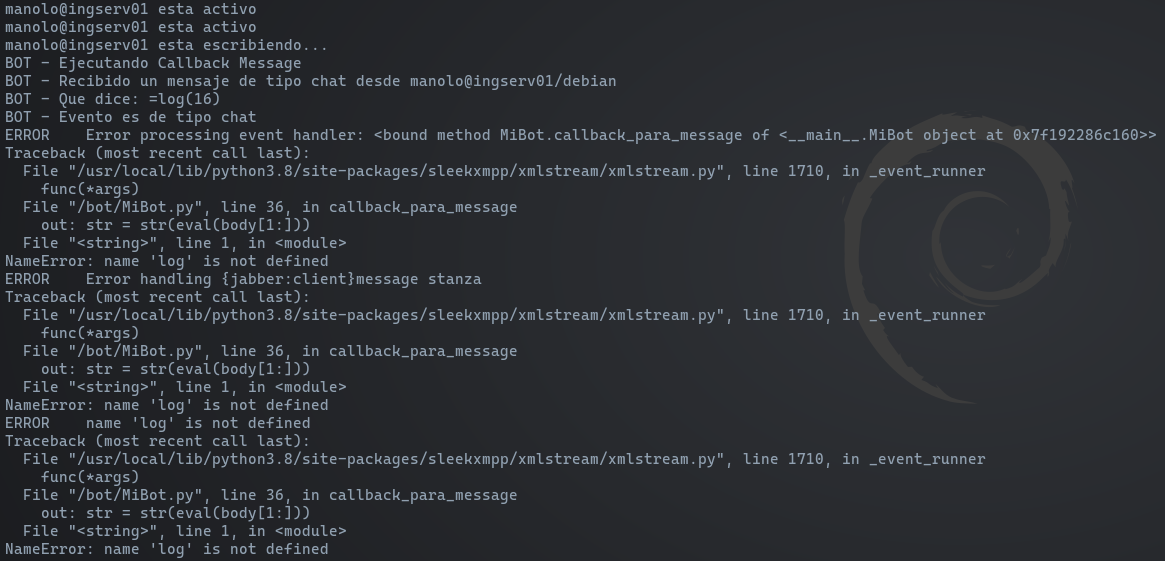
\includegraphics[width=\textwidth]{6/Imagen616.png}
	\captionof{figure}{Excepción en el bot al usar $log$}\label{fig:6/7}
\end{minipage}

\section{Conclusiones}

Esta práctica resulta ser de las más interesantes ya que permite al alumno conocer una Introducción
a un protocolo que puede ser utilizado en muchos casos.

El caso de uso más obvio (el mismo utilizado en esta práctica) es lógicamente una aplicación de
mensajería. No obstante, sería posible también utilizar XMPP para diseñar una red de sistemas
que se puedan comunicar entre sí. Si bien no es necesario utilizar XMPP para cumplir este objetivo,
puede facilitar muchas de las comunicaciones que podrían ser necesarias en dicha red
(como por ejemplo que dos sistemas se subscriban a las notificaciones de otro).

Respecto a Pidgin, afortunadamente es una aplicación que está disponible en diversos sistemas operativos
por lo que no fue complicado instalarla en Debian (cosa que no se puede esperar de la mayoría de asignaturas).
Por otro lado, Pidgin resulta un poco incómodo de utilizar debido principalmente a su uso de diversas ventanas.
Existe una ventana para hacer login, otra para el listado de amigos, otra para añadir amigos nuevos,
otra para cada chat\dots Aunque para la duración de la práctica, no es un inconveniente destacable.

Hubiese sido interesante (comprendemos que no se ha realizado por falta de tiempo) desarrollar una
aplicación que utilice el protocolo XMPP.
Esto es, diseñar un 'Pidgin' casero.
No hay duda que quedará en la lista de proyectos por hacer de muchos alumnos.

Respecto al desarrollo del bot, en nuestro caso hemos invertido una mayor cantidad de tiempo depurando
problemas relacionados con SSL que desarrollando el bot en sí.
Es interesante dar a conocer cómo crear un bot en XMPP, pero en nuestra experiencia no ha sido particularmente
eficiente.

Los problemas del desarrollo del bot se originan principalmente de la no disponibilidad de la libería
\verb#sleekxmpp# y de los problemas con SSL.

\begin{notebox}
	No tenemos en cuenta los problemas relacionados con \verb#sleekxmpp# ni SSL debido a que seguramente
	sean causados por utilizar operativos distintos a los especificados en la guía docente de
	la asignatura.

	Ningún otro alumno de nuestro grupo de prácticas se ha encontrado con estos problemas.
\end{notebox}

\begin{center}
	\begin{tabular}{|c|c|}
		\hline
		\textbf{Autor} & \textbf{Porcentaje} \\
		\hline
		\hline
		\authorOne & 10\% \\
		\authorTwo & 90\% \\
		\hline
	\end{tabular}
\end{center}